\label{sec:det}
In the ET approach, starting from an initiating event (i.e. accident event), several final outcomes are forecasted by assembling ``all'' combinations of events that might follow. This leads to the classical tree structure. The probability of a specific outcome (branch) is given by the product of the events along that branch.
Two of the disadvantages of these methods are that, first timing/sequencing of events and system dynamics are not explicitly accounted for in the analysis and second the status and behavior of the system has no influence on the likelihood of the events.
%A PRA analysis needs an approximation to this distribution for selected consequence variables.
%A way to achieve this goal is through a DET approach.
\begin{figure}[h]
  \centering
     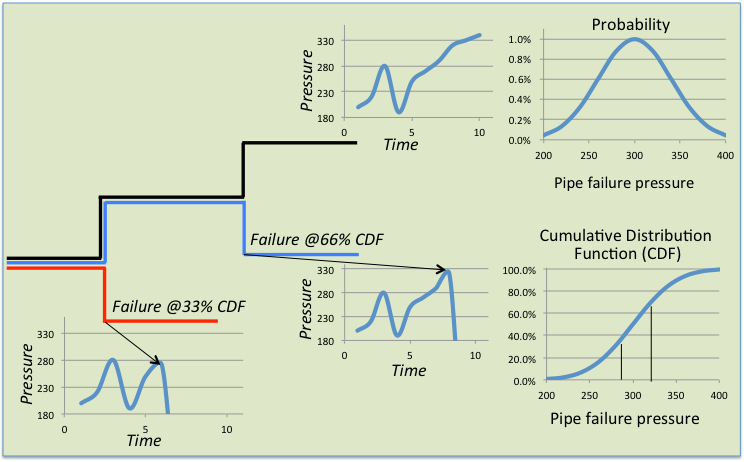
\includegraphics[width=0.73\textwidth]{figures/DET_schemeFlow.png}
  \caption{Dynamic Event Tree Conceptual Scheme.}
   \label{fig:DET_schemeFlow}
\end{figure}
In order to overcome these limitations a ``dynamic'' approach is needed. The DET technique brings several advantages~\cite{alfonsiPSA}~\cite{ADAPTHakobyan}, among which the fact that it simulates probabilistic system evolution in a way that is consistent time evolution of the accident scenario. In DET,  event sequences are run simultaneously starting from a single initiating event. The branchings occur at user specified times/conditions and/or when an action is required by the operator and/or the system, creating a deterministic sequence of events based on the time of their occurrence (see Fig.~\ref{fig:DET_schemeFlow}).

This leads to a more realistic and mechanistically consistent analysis of the considered system. DPRA, including  DET methodologies,  are designed to take the timing of events explicitly into account, which can become very important especially when uncertainties associated to complex phenomena are considered. \\
The main idea of this methodology is to let a system code (i.e., RELAP-7) determine the pathway of an accident scenario within a probabilistic ``environment''.

From a simulation point of view, a DET analysis starts with a single simulation that, most likely, represents the NPP immediately after an initiating event (an event that may lead to a risky state of the NPP). Every time the simulation faces an event affected by a probabilistic behavior (e.g. failure of a relief valve, etc.), several simulation branches are spawned. Each simulation accounts for a fraction of the possible outcomes.
Figure~\ref{fig:DET_schemeFlow} exemplifies this approach. After an initiating event, the simulation follows the accident sequence and a pipe is affected by a probability of failure described by a \textbf{P}robabilistic \textbf{D}istribution \textbf{F}unction (i.e. pipe failure probability as function of the internal pressure) and a corresponding \textbf{C}umulative \textbf{D}istribution \textbf{F}unction (\textbf{CDF}).
In addition, the user provides a grid of probability thresholds for the CDF. Every time the simulation detects a pressure corresponding to a threshold in the probability grid, a new set of simulation branches is generated (ie., a branch  where the pipe is damaged  and another where nothing happened).

In general each sequence continues until another event occurs and a new set of branches is spawned. The simulation ends when an exit condition or a maximum mission time is reached.
